\documentclass[a4paper,12pt]{article}
\usepackage[utf8]{inputenc}
\usepackage[english]{babel}
\usepackage{graphicx}
\usepackage{amsmath}
\usepackage{geometry}
 \geometry{
 a4paper,
 total={170mm,257mm},
 left=20mm,
 top=20mm,
 }
\newcommand{\page}[1]{\footnotesize{(p.{#1})}}

%Beginning of the document
\begin{document}
\section*{Formula Booklet - Essentials}
\subsection*{Trigonometric}
\begin{equation*}
  \begin{split}
    \sin(A \pm B) &= \sin{A}\cos{B}\pm\cos{A}\sin{B}\\
    \cos(A \pm B) &= \cos{A}\cos{B}\mp\sin{A}\sin{B}\\\\
    e^{ix} &= \cos(x) + i\sin(x)
  \end{split}
\end{equation*}
$$\cos{x} = \frac{e^{ix} + e^{-ix}}{2},\hspace{5mm}\sin{x} = \frac{e^{ix} - e^{-ix}}{2i}$$

\subsection*{Hyperbolic}
\begin{equation*}
  \begin{split}
    \sinh(A \pm B) &= \sinh{A}\cosh{B}\pm\cosh{A}\sinh{B}\\
    \cosh(A \pm B) &= \cosh{A}\cosh{B}\pm\sinh{A}\sinh{B}\\
  \end{split}
\end{equation*}
$$\cosh{x} = \frac{e^x+e^{-x}}{2} ,\hspace{5mm}\sinh{x} = \frac{e^x-e^{-x}}{2}$$
\begin{figure}[h]
  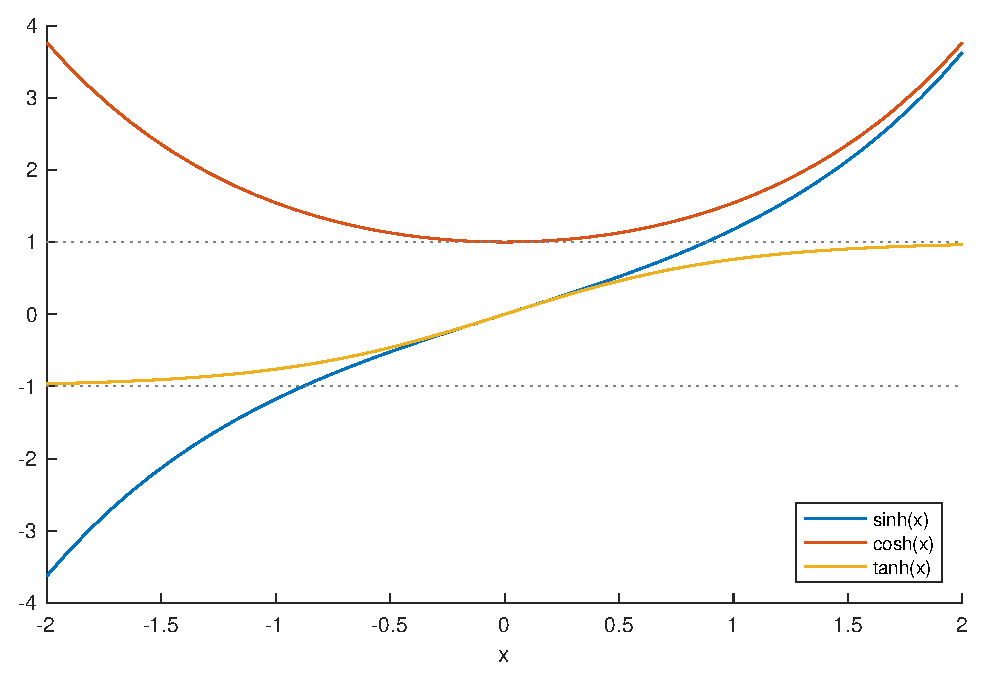
\includegraphics[width=0.8\textwidth]{hyperbolic_figures.eps}
  \centering
\end{figure}


\subsection*{Quotient rule}
$$f(x) = \frac{u(x)}{v(x)} \hspace{3mm}\Rightarrow\hspace{3mm} f'(x) = \frac{vu'-uv'}{v^2}$$

\subsection*{Integrating factor}
$$\frac{dy}{dx}+P(x)y = R(x,y) \hspace{3mm}\Rightarrow\hspace{3mm} I(x) = \exp\left(\int P(x)dx\right)$$

\subsection*{Taylor Series}
\begin{align*}
  f(x) &= \sum_{n=0}^\infty \frac{f^{(n)}(a)}{n!}(x-a)^n \\
  &= f(a) + f'(a)(x-a) + \frac{f''(a)}{2!}(x-a)^2+\cdots
\end{align*}

\subsection*{Residue at n-th order pole at $k=k_0$}
$$Res(f,k_0)=\frac{1}{(n-1)!}\lim_{k\to k_0} \frac{d^{n-1}}{dk^{n-1}}\bigg((k-k_0)^n f(k)\bigg)$$
so for a simple-pole (n=1), we have
$$Res(f,k_0)=\lim_{k\to k_0}(k-k_0)f(k)$$

\subsection*{Contour integration (with n-th order pole at $k=k_0$)}
$$\int_C f(x)dx = \left\{ \begin{tabular}{ll}
  $2\pi i \times Res(f,k_0)$ & if $C$ counter-clockwise\\
  $-2\pi i \times Res(f,k_0)$ & if $C$ clockwise\\
\end{tabular}
\right.$$

\subsection*{Integrals}
\begin{equation*}
  \begin{split}
    \int \frac{a}{a^2+x^2}dx &= \tan^{-1}\left(\frac{x}{a}\right)\\
    \int \frac{1}{\sin{x}}dx &= \log\left|\tan\left(\frac{x}{2}\right)\right|\\
    \int \frac{1}{\cos{x}}dx &= \log\left|\sec(x)+\tan(x)\right|
  \end{split}
\end{equation*}

\subsection*{Heaviside function}
$$H(x) = \left\{ \begin{tabular}{cc}
  $1$ & if $x>0,$ \\
  $0$ & if $x<0.$

\end{tabular} \right.$$

\subsection*{Dirac delta function}
$$\delta(x) = \left\{ \begin{tabular}{cc}
  $\infty$ & if $x=0,$ \\
  $0$ & if $x\neq 0.$
\end{tabular} \right. \hspace{5mm} \text{where} \hspace{5mm}\int^\infty_{-\infty} \delta(x)dx = 1$$


\end{document}
